% 图 6.16 中子三轴谱仪示意图：反应堆-准直器-单色器(旋转屏蔽)-样品(2theta)-分析器-探测器
\documentclass[tikz,border=5pt]{standalone}
\usetikzlibrary{arrows.meta,calc}
\usepackage{amsmath}
\usepackage{bm}
\usepackage{fontspec}
\setmainfont{Times New Roman}
\begin{document}
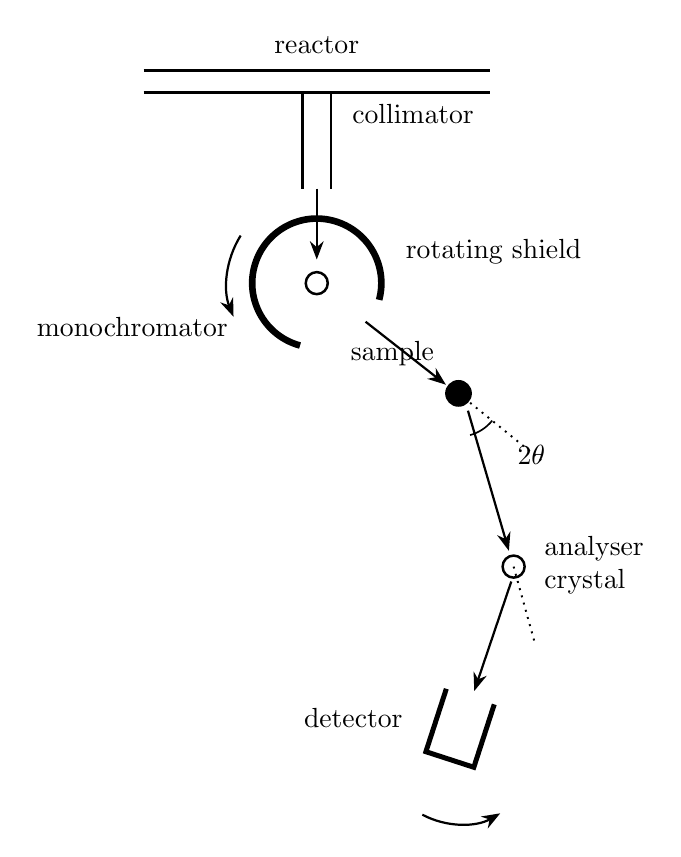
\begin{tikzpicture}[line width=0.8pt,>=Stealth]
% ---------- reactor (double line) ----------
\draw[line width=0.9pt] (0.3,7.6) -- (4.7,7.6);
\draw[line width=0.9pt] (0.3,7.32) -- (4.7,7.32);
\node[anchor=south] at (2.5,7.68) {reactor};
% ---------- collimator (channel) ----------
\draw (2.32,7.32) -- (2.32,6.1);
\draw (2.68,7.32) -- (2.68,6.1);
\node[anchor=west] at (2.82,7.05) {collimator};
% beam: collimator -> monochromator
\draw[->] (2.5,6.1) -- (2.5,5.2);
% ---------- rotating shield around monochromator ----------
\coordinate (mono) at (2.5,4.9);
\draw[line width=2.4pt] ([shift={(mono)}]-15:0.82) arc[start angle=-15,end angle=255,radius=0.82];
\draw[->,line width=0.8pt] ([shift={(mono)}]148:1.14) arc[start angle=148,end angle=202,radius=1.14];
\node[anchor=west] at (3.5,5.3) {rotating shield};
\node[anchor=east] at (1.5,4.35) {monochromator};
% monochromator crystal (open circle)
\draw[fill=white,line width=0.9pt] (mono) circle (0.14);
% ---------- beam: monochromator -> sample ----------
\coordinate (samp) at (4.3,3.5);
\draw[->] (3.12,4.41) -- (4.14,3.61);
% sample (filled)
\fill (samp) circle (0.17);
\node[anchor=south east] at (4.12,3.72) {sample};
% dotted extension of incident beam + 2theta arc
\draw[dotted,line width=0.7pt] (samp) -- ++(-39:1.35);
\draw[line width=0.6pt] ([shift={(samp)}]-74.5:0.55) arc[start angle=-74.5,end angle=-39,radius=0.55];
\node[anchor=west] at (4.92,2.72) {$2\theta$};
% ---------- beam: sample -> analyser ----------
\coordinate (ana) at (5.0,1.3);
\draw[->] (4.42,3.28) -- (4.94,1.5);
% analyser crystal (open circle)
\draw[fill=white,line width=0.9pt] (ana) circle (0.14);
\node[anchor=west,align=left] at (5.26,1.32) {analyser\\crystal};
\draw[dotted,line width=0.7pt] (ana) -- ++(-74.5:1.0);
% ---------- beam: analyser -> detector ----------
\draw[->] (4.97,1.11) -- (4.5,-0.28);
% detector: tilted trough (open towards beam)
\begin{scope}[shift={(4.32,-0.75)},rotate=-18]
  \draw[line width=1.8pt] (-0.32,0.42) -- (-0.32,-0.42) -- (0.32,-0.42) -- (0.32,0.42);
\end{scope}
\node[anchor=east] at (3.72,-0.62) {detector};
% rotation arc under detector
\draw[->,line width=0.8pt] ([shift={(4.32,-0.95)}]242:1.02) arc[start angle=242,end angle=300,radius=1.02];
\end{tikzpicture}
\end{document}
